%%%%%%%%%%%%%%%%%%%%%%%%%%%%%%%%%%%%%%%%%%%%%%%%%%%%%%%%%%%%%%%%%%%%%%%
% BAB 4
%%%%%%%%%%%%%%%%%%%%%%%%%%%%%%%%%%%%%%%%%%%%%%%%%%%%%%%%%%%%%%%%%%%%%%%




% question: perancangan model? atau digabung dengan tahap pelatihan model?


\mychapter{4}{BAB 4 PERANCANGAN SISTEM}

Pada bab ini, akan dijelaskan tahap-tahap yang dilakukan dalam perancangan sistem klasifikasi detak jantung yang digunakan dalam penelitian ini.
Perancangan sistem meliputi tahap \textit{preprocessing} data, ekstraksi fitur, perancangan model LSTM, pelatihan model, dan evaluasi model.
Gambar \ref{fig:alur-sistem} menunjukkan alur perancangan sistem yang digunakan dalam penelitian ini.

%
\begin{figure}[H]
  \begin{center}
    \includegraphics[width=1\textwidth]{img/lstm-ML Pipeline.drawio.pdf}
  \end{center}
  \caption{Alur perancangan sistem}
  \label{fig:alur-sistem}
\end{figure}

\section{\emph{Preprocessing} Data}
\label{subsec: bab4-preprocessing-data}
 
Dataset yang digunakan dalam penelitian ini diperoleh dari MIT-BIH Arrhythmia Database.
% Sebelum data dapat digunakan untuk pelatihan model, data ECG harus melalui tahap \textit{preprocessing}.
% \textit{Preprocessing} dilakukan untuk memastikan kualitas dan keandalan data yang digunakan dalam proses pelatihan model. 
% Terdapat beberapa tahap \textit{preprocessing} yang dilakukan pada penelitian ini, yaitu pemetaan dataset, penghapusan \textit{noise} berfrekuensi tinggi, penghapusan \textit{baseline wander} (BW), dan normalisasi.
Data ECG pada MIT-BIH Arrhythmia Database memiliki anotasi yang terdiri dari 20 kelas, sedangkan pada penelitian ini hanya menggunakan 5 kelas, yaitu Normal (N), \textit{Supraventricular Ectopic Beat} (S), \textit{Ventricular Ectopic Beat} (V), \textit{Fusion} (F), dan \textit{Unknown} (Q).
Kelas-kelas tersebut dipilih berdasarkan rekomendasi dari Association for the Advancement of Medical Instrumentation (AAMI), yang mengelompokkan berbagai jenis aritmia ke dalam kategori yang lebih umum.
Oleh karena itu, perlu dilakukan pemetaan kelas pada dataset agar sesuai dengan kelas yang digunakan pada penelitian ini.
Pemetaan tersebut dapat dilihat pada Tabel \ref{tab:aami-label}, yang menunjukkan bagaimana kelas-kelas dari dataset dipetakan ke dalam 5 kelas yang digunakan dalam penelitian ini.

\begin{table}[h]
	\caption{Kelas rekomendasi AAMI dan simbol pada MIT-BIH}
	\begin{center}
		\begin{tabular}{|l @{\hspace{1cm}} |l|}
			\hline
			% \textbf{AAMI}                              & \textbf{MIT-BIH}       \\
			\multicolumn{1}{|c|}{\textbf{AAMI}} & \multicolumn{1}{c|}{\textbf{MIT-BIH}} \\
			\hline
			Normal (N)                        & N, L, R, e, j \\
			\hline
                        \textit{Supraventricular Ectopic Beat} (S) & A, a, J, S    \\
			\hline
                        \textit{Ventricular Ectopic Beat} (V)      & V, E          \\
			\hline
                        \textit{Fusion} (F)                        & F             \\
			\hline
                        \textit{Unknown} (Q)                       & /, f, Q       \\
			\hline
		\end{tabular}
	\end{center}
	\label{tab:aami-label}
\end{table}

% table count
% 0    86399
% 2     6512
% 1     2692
% 3      787
% 4        8

Jumlah data pada setiap kelas setelah dilakukan pemetaan dapat dilihat pada Tabel \ref{tab:count-label}.
Jumlah seluruh detak jantung pada dataset yang digunakan dalam penelitian ini adalah 96398 detak.
Dari tabel tersebut dapat dilihat bahwa kelas Normal (N) memiliki jumlah data terbanyak dengan jumlah 86399 data.
Sementara itu, kelas \textit{Unknown} (Q) memiliki jumlah data terendah dengan jumlah 8 data.
% Terdapat ketidakseimbangan kelas yang cukup signifikan pada dataset, dengan kelas minoritas yang memiliki jumlah kurang dari 1\% dari kelas mayoritas.
Terdapat ketidakseimbangan kelas yang cukup signifikan pada dataset.
Kelas minoritas, yaitu \textit{Unknown} (Q), memiliki jumlah data kurang dari 1\% dari kelas mayoritas.


\begin{table}[H]
  \caption{Jumlah data pada setiap kelas}
  \begin{center}
    \begin{tabular}{|l @{\hspace{1cm}} |c|}
      \hline
      % \textbf{Kelas} & \textbf{Jumlah Data} \\
      \multicolumn{1}{|c|}{\textbf{Kelas}} & \multicolumn{1}{c|}{\textbf{Jumlah Data}} \\
      \hline
      Normal (N)                        & 86399 \\
      \hline
      \textit{Supraventricular Ectopic Beat} (S) & 2692  \\
      \hline
      \textit{Ventricular Ectopic Beat} (V)      & 6512  \\
      \hline
      \textit{Fusion} (F)                        & 787   \\
      \hline
      \textit{Unknown} (Q)                       & 8     \\
      \hline
      % \textbf{Jumlah Total} & 96398 \\
      \multicolumn{1}{|c|}{\textbf{Jumlah Total}} & \multicolumn{1}{c|}{96398} \\
      \hline
    \end{tabular}
  \end{center}
  \label{tab:count-label}
\end{table}

% % metode penghilangan frekuensi tinggi
% %     ecg = denoise_wavelet(ecg, method='VisuShrink', mode='soft', wavelet_levels=10, wavelet='db8', rescale_sigma='True')
%
% Selama proses pengambilan data, sinyal ECG rentan terhadap \textit{noise} berfrekuensi tinggi.
% Frekuensi tinggi pada data ECG dianggap sebagai \textit{noise} yang dapat mengganggu proses klasifikasi detak jantung, sehingga perlu dilakukan penghilangan \textit{noise} tersebut.
% Pada penelitian ini, \textit{noise} berfrekuensi tinggi dihilangkan dengan menggunakan metode \textit{wavelet denoise}.
% \textit{Wavelet denoise} merupakan metode yang digunakan untuk menghilangkan \textit{noise} pada sinyal maupun gambar dengan menggunakan \textit{wavelet transform}.
% \textit{Wavelet transform} memungkinkan sinyal untuk dipecah menjadi beberapa bagian frekuensi yang berbeda, sehingga memungkinkan penghilangan \textit{noise} pada frekuensi tertentu.
% Metode \textit{wavelet denoise} yang digunakan pada penelitian ini adalah \textit{VisuShrink} dengan mode \textit{soft thresholding}, dan menggunakan \textit{wavelet} Daubechies 8 (db8) dengan 10 level \textit{wavelet decomposition}.
%
% % --- dijelaskan lebih detail? ---
%
% % Sinyal ECG diubah ke dalam domain \textit{wavelet} dengan menggunakan \textit{wavelet transform} Daubechies 8 (db8) dengan 10 level \textit{wavelet decomposition}.
% % \textit{Noise} pada sinyal ECG kemudian dapat dihilangkan dengan mengurangi koefisien \textit{wavelet} yang memiliki nilai di bawah ambang batas tertentu.
%
% %
% % Setelah menghilangkan \textit{noise} berfrekuensi tinggi, tahap selanjutnya adalah menghilangkan \textit{baseline wander} (BW).
% % elaborate
% Selain \textit{noise} berfrekuensi tinggi, sinyal ECG juga rentan terhadap \textit{baseline wander}.
% \textit{Baseline wander} (BW) merupakan \textit{noise} berfrekuensi rendah yang terdapat pada ECG.
% BW dapat disebabkan oleh beberapa faktor, seperti pernapasan, elektroda yang bermuatan listrik, dan gerakan dari pasien \parencite{lenisComparisonBaselineWander2017}.
% % metode baseline wander
%         % baseline = medfilt(ecg, 71)
%         % baseline = medfilt(baseline, 215)
%         %
%         % # Remove Baseline
%         % for i in range(0, len(ecg)):
%         %     ecg[i] = ecg[i] - baseline[i]
% % BW dihilangkan dengan menggunakan metode \textit{median filter} dengan panjang jendela 71 dan 215.
% BW dihilangkan dengan melakukan substraksi antara sinyal ECG dengan \textit{trend} sinyal.
% \textit{Trend} sinyal diperoleh dengan menggunakan metode \textit{median filter} sebanyak dua kali dengan panjang jendela 71 dan 215.
% % Median filtering, as mentioned earlier, is another method commonly used for baseline wander removal. It involves replacing each data point in the signal with the median value within a specified window around that point. This approach can effectively remove baseline variations while preserving the shape of the ECG waveform.
% \textit{Median filter} akan menggantikan setiap titik data pada sinyal dengan nilai median dalam jendela yang ditentukan.
% \textit{Median filter} didefinisikan oleh persamaan \ref{eq:median-filter}
% \begin{equation}
%     % perlu dicek lagi
%     y[n] = \text{median}(x[n - \frac{M}{2} : n + \frac{M}{2}])
%     \label{eq:median-filter}
% \end{equation}
% dengan $y[n]$ adalah sinyal hasil \textit{median filter}, $x[n]$ adalah sinyal asli, dan $M$ adalah panjang jendela \textit{median filter}.
% % Yang mana $y[n]$, $x[n]$, dan $M$ masing-masing menunjukkan sinyal hasil \textit{median filter}, sinyal asli, dan panjang jendela \textit{median filter}.
%
% % Setelah \textit{baseline wander} dihilangkan, data dinormalisasi untuk menghindari perbedaan skala.
% % Setelah \textit{nose} dan \textit{baseline wander} dihilangkan, data dinormalisasi untuk menghindari perbedaan skala.
% % Normalisasi yang dilakukan yaitu \textit{Z-score normalization}.
% % metode normalisasi
% Setelah \textit{noise} dan \textit{baseline wander} dihilangkan, tahap selanjutnya adalah normalisasi data.
% Normalisasi dilakukan untuk menghindari adanya perbedaan skala pada data.
% Metode normalisasi yang digunakan pada penelitian ini adalah \textit{Z-score normalization}.
% \textit{Z-score normalization} mengubah data ke dalam distribusi normal dengan rata-rata 0 dan standar deviasi 1.
% \textit{Z-score normalization} didefinisikan oleh persamaan \ref{eq:z-score}
% \begin{equation}
% 		z = \frac{x - \mu}{\sigma}
% 		\label{eq:z-score}
% \end{equation}
% dengan $z$ adalah data yang telah dinormalisasi, $x$ adalah data asli, $\mu$ adalah rata-rata data, dan $\sigma$ adalah standar deviasi data.
%
%
% % Gambar \ref{fig:sebelum-prep} menunjukkan data sebelum dilakukan \textit{preprocessing}, sedangkan Gambar \ref{fig:setelah-prep} menunjukkan data setelah dilakukan \textit{preprocressing}.
% Gambar \ref{fig:sebelum-prep} dan \ref{fig:setelah-prep} memperlihatkan perbandingan data ECG sebelum dan setelah dilakukan \textit{preprocessing}.
% % Pada Gambar \ref{fig:sebelum-prep}, terlihat bahwa terdapat \textit{noise} berfrekuensi tinggi dan variasi pada \textit{baseline} sinyal ECG.
% Pada Gambar \ref{fig:sebelum-prep}, terlihat bahwa pada data ECG masih terdapat gangguan seperti \textit{noise} berfrekuensi tinggi dan variasi pada \textit{baseline} sinyal.
% % Setelah dilakukan \textit{preprocessing}, sinyal ECG menjadi lebih halus dan memiliki baseline yang lebih rata.
% Setelah dilakukan \textit{preprocessing}, sinyal ECG menjadi lebih halus dan memiliki \textit{baseline} yang lebih rata, seperti yang terlihat pada Gambar \ref{fig:setelah-prep}.
%
% \begin{figure}[H]
%     \centering
%     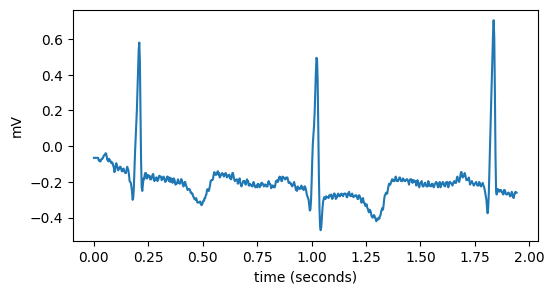
\includegraphics[width=0.6\linewidth]{./img/sebelum_prep.png}
% 	\caption{Data sebelum \textit{preprocessing}}
% 	\label{fig:sebelum-prep}
% \end{figure}
%
% \begin{figure}[H]
%   \centering
%   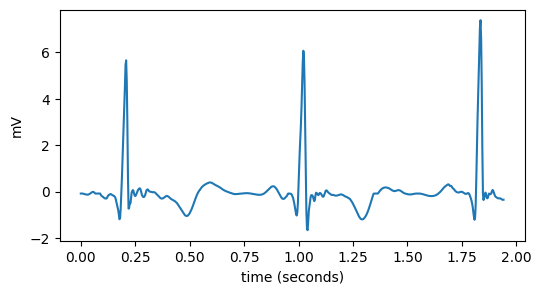
\includegraphics[width=0.6\linewidth]{./img/setelah_prep.png}
%   \caption{Data setelah \textit{preprocessing}}
%   \label{fig:setelah-prep}
% \end{figure}
%

\section{Ekstraksi Fitur}
\label{subsec: bab4-ekstraksi-fitur}

% Kami menggunakan RR-Interval sebagai fitur dalam penelitian ini.
% taruh sini atau bab 2?
% RR-Interval adalah jarak antara dua titik R pada sinyal ECG, yang merepresentasikan interval antara dua detak jantung.
% Visualisasi dari RR-Interval ditunjukkan oleh Gambar \ref{fig:rri}.
% Dalam gambar tersebut, terdapat puncak 'R' yang menandakan titik maksimum voltase selama siklus detak jantung pada sinyal ECG.
% Jarak antara dua puncak 'R' ini menunjukkan RR-Interval yang menjadi fitur utama dalam penelitian ini.
% \begin{figure}[H]
%   \centering
%   \includegraphics[scale=.7]{img/lstm-Page-7.drawio.pdf}
%   \caption{RR-Interval}
%   \label{fig:rri}
% \end{figure}

% --- pindah ke bab 2? ---

Fitur utama yang digunakan dalam penelitian ini adalah RR-Interval.
Pada dataset MIT-BIH Arrhythmia Database, sudah terdapat anotasi R-peak yang menunjukkan posisi puncak 'R' pada sinyal ECG.
Dari posisi R-peak tersebut, dapat dihitung jarak antara dua puncak 'R' untuk mendapatkan RR-Interval.
RR-Interval dihitung dengan menggunakan persamaan \ref{eq:rr-interval}
% RRi[i] = Rpeak[i+1] - Rpeak[i]
\begin{equation}
		RRi[i] = Rpeak[i+1] - Rpeak[i]
		\label{eq:rr-interval}
\end{equation}
dengan $RRi[i]$ adalah RR-Interval ke-$i$, dan $Rpeak[i]$ adalah posisi R-peak ke-$i$.
RR-Interval tersebut kemudian diekstraksi menjadi 9 fitur, yaitu RR0, RR-1, RR+1, RR0/avgRR, tRR0, RR-1/avgRR, RR-1/RR0, RR+1/avgRR, dan RR+1/RR0 \parencite{pramukantoroHeartbeatClassifierContinuous2022}.
Tabel \ref{tab:rri} menunjukkan deskripsi lengkap dari setiap fitur yang digunakan dalam penelitian ini.
Ekstraksi dilakukan dengan menggunakan jendela sepanjang 42 data. 
        % avgRR = np.mean(rr_intervals[i-42:i+1])
        % stddevRR = np.std(rr_intervals[i-42:i+1])
% Rata-rata RR-Interval (avgRR) merupakan rata-rata dari 42 data, termasuk RR-0. 
Rata-rata RR-Interval (avgRR) dan standar deviasi RR-Interval (stddevRR) dihitung dengan menggunakan persamaan \ref{eq:avg-rr} dan \ref{eq:stddev-rr}.
\begin{equation}
		\text{avgRR} = \frac{1}{42} \sum_{i=0}^{42} RRi[i]
		\label{eq:avg-rr}
\end{equation}
\begin{equation}
		\text{stddevRR} = \sqrt{\frac{1}{42} \sum_{i=0}^{42} (RRi[i] - \text{avgRR})^2}
		\label{eq:stddev-rr}
\end{equation}


\begin{table}[H]
  \caption{Deskripsi RR-Interval}
\begin{center}
\footnotesize
\begin{tabular}{|l @{\hspace{1cm}} |l|}
\hline
% \textbf{Fitur} & \textbf{Deskripsi}\\
\multicolumn{1}{|c|}{\textbf{Fitur}} & \multicolumn{1}{c|}{\textbf{Deskripsi}}\\
\hline
RR0 & Nilai RRi saat ini\\
\hline
RR-1 & Nilai RRi sebelumnya\\
\hline
RR+1  & Nilai RRi selanjutnya\\
\hline
RR0/avgRR & Nilai RRi saat ini dibagi dengan rata-rata 42 RRi sebelumnya\\
\hline
tRR0  & (RRi saat ini - rata-rata RRi) / stddevRRi\\
\hline
RR-1/avgRR & Nilai RRi sebelumnya / rata-rata RRi\\
\hline
RR-1/RR0 & Nilai RRi sebelumnya / RRi saat ini\\
\hline
RR+1/avgRR & Nilai RRi selanjutnya / rata-rata RRi\\
\hline
RR+1/RR0 & Nilai RRi selanjutnya / RRi saat ini\\
\hline
\end{tabular}
\end{center}
\center
Sumber: \textcite{pramukantoroHeartbeatClassifierContinuous2022}
\label{tab:rri}
\end{table}

%contoh extracted feature

% considering cuma pakai lstm256 tapi dengan fitur lain
\section{Perancangan Model LSTM}
\label{subsec: bab4-pembuatan-model-lstm}
% Pada tahap ini, penulis membuat model berbasis LSTM yang akan digunakan untuk melakukan klasifikasi detak jantung. 
% Dalam penelitian ini, 
% Pembuatan model meliputi pembuatan arsitektur model, pelatihan model, dan evaluasi model.
% Model dibuat dengan menggunakan \textit{framework} TensorFlow dan dilatih sebanyak 50 \textit{epoch}.


% LSTM merupakan pengembangan dari \textit{Recurrent Neural Network} (RNN) yang dirancang untuk mengatasi masalah yang umum terjadi pada RNN tradisional, yaitu hilangnya informasi masa lalu \parencite{hochreiterLongShorttermMemory1997}.  LSTM memiliki kemampuan untuk mengingat informasi yang disimpan dalam jangka waktu yang lama. 


Terdapat tiga jenis model yang akan digunakan pada penelitian, yaitu \textit{Long Short-Term Memory} (LSTM), \textit{Bidirectional} LSTM (Bi-LSTM), serta LSTM \textit{Fully Convolutional Network} (LSTM-FCN). 
Arsitektur model LSTM yang digunakan dalam penelitian ini ditunjukkan oleh Gambar \ref{fig:arslstm}. Model terdiri dari tiga \textit{layer}, yakni satu buah LSTM \textit{layer} dan dua buah \textit{dense layer}. 
% Terdapat dua varian model LSTM yang dilatih dengan menggunakan dua \textit{hyperparameter} berbeda.
% Terdapat dua varian model LSTM dengan menggunakan dua \textit{hyperparameter} berbeda.
Dalam penelitian ini, digunakan dua model LSTM dengan \textit{hyperparameter} yang berbeda.
Model pertama memiliki 512 unit LSTM pada \textit{layer} pertama dan 256 unit \textit{dense} pada \textit{layer} kedua. Sementara itu, model kedua memiliki 256 unit LSTM pada layer pertama dan 128 unit \textit{dense} pada \textit{layer} kedua.

% img arsi lstm
\begin{figure}[H]
  \centering
  \includegraphics[scale=.9, angle=-90]{img/lstm-Page-2.drawio.pdf}
  \caption{Arsitektur LSTM}
  \label{fig:arslstm}
\end{figure}

\textit{Bidirectional} LSTM atau Bi-LSTM merupakan pengembangan dari LSTM yang dapat dilatih dua arah secara bersamaan dengan \textit{hidden layer} yang terpisah \parencite{yuReviewRecurrentNeural2019}. Dengan menggabungkan LSTM dengan \textit{bidirectional} RNN, Bi-LSTM mampu mengatasi keterbatasan LSTM konvensional yang hanya dapat memanfaatkan informasi sebelumnya. Gambar \ref{fig:arsbilstm} menunjukkan arsitektur model Bi-LSTM yang digunakan dalam penelitian ini.
Arsitektur yang digunakan sama dengan arsitektur pada model LSTM, hanya saja \textit{layer} LSTM diganti dengan \textit{bidirectional} LSTM.
\textit{Hyperparameter} yang digunakan pada model Bi-LSTM adalah 256 unit Bi-LSTM pada \textit{layer} pertama dan 256 unit \textit{dense} pada \textit{layer} kedua.

% img arsi bi-lstm
\begin{figure}[H]
  \centering
  \includegraphics[scale=.9, angle=-90]{img/lstm-Page-3.drawio.pdf}
  \caption{Arsitektur Bi-LSTM}
  \label{fig:arsbilstm}
\end{figure}

LSTM-FCN atau LSTM-\textit{Fully Convolutional Network} merupakan model gabungan antara LSTM dengan  \textit{Fully Convolutional Network} (FCN) \parencite{karimLSTMFullyConvolutional2018}.
Arsitektur model ini terdiri dari dua blok, yaitu blok \textit{convolutional} dan blok LSTM.
% conv1d (128) -> conv1d (256) -> conv1d (128) -> global pooling
Blok \textit{convolutional} terdiri dari tiga \textit{layer convolutional} 1 dimensi dengan jumlah filter berturut-turut 128, 256, dan 128.
% Output dari tiga \textit{layer convolutional} tersebut diambil dengan menggunakan \textit{global average pooling}.
Kemudian, keluaran dari tiga \textit{layer convolutional} tersebut diambil dengan menggunakan \textit{global average pooling}.
% , sedangkan blok LSTM hanya terdiri dari satu layer LSTM.
Sementara itu, blok LSTM hanya terdiri dari satu \textit{layer} LSTM dengan ukuran 8 unit.
% Pada LSTM-FCN, untuk menghindari \textit{overfitting}, terdapat \textit{dimension shuffle} yang akan mengacak input sebelum blok LSTM.
% Pada LSTM-FCN, \textit{dimension shuffle} digunakan untuk menghindari \textit{overfitting} dengan mengacak input sebelum blok LSTM.
% Akan tetapi, meletakkan \textit{dimension shuffle} sebelum blok LSTM akan menyebabkan hilangnya informasi pada dimensi waktu \parencite{8713870}.
% Pada penelitian ini kami melakukan modifikasi pada LSTM-FCN dengan menukar posisi \textit{dimension shuffle} pada sebelum blok \textit{convolutional}.
% Gambar \ref{fig:arslstmfcn} menunjukkan struktur model LSTM-FCN modifikasi yang digunakan pada penelitian.
% Dalam penelitian ini, dilakukan modifikasi pada LSTM-FCN dengan memindahkan \textit{dimension shuffle} dari posisinya sebelum blok LSTM ke sebelum blok \textit{convolutional}.
Dalam penelitian ini, \textit{dimension shuffle} diposisikan pada sebelum blok \textit{convolutional}.
Gambar \ref{fig:arslstmfcn} menunjukkan struktur model LSTM-FCN yang digunakan pada penelitian.

% img arsi lstm-fcn
\begin{figure}[H]
  \centering
  \includegraphics[scale=0.7, angle=-90]{img/lstm-Page-4.drawio.pdf}
  \caption{Arsitektur LSTM-FCN Modifikasi}
  \label{fig:arslstmfcn}
\end{figure}

\section{Pelatihan Model}
% [60479  1884  4558   551     6]
% model.compile(loss='categorical_crossentropy',
% 		optimizer='adam',
% 		metrics=['accuracy'])
%
% history = model.fit(X_train, y_train,epochs=50, batch_size=256, verbose=1)

% --- loss: categorical crossentropy, optimizer: adam, learning rate: 0.001, batch size: 256, epoch: 50, dgx a100 ---
Seluruh model dilatih dengan menggunakan \textit{framework} TensorFlow. 
% Pelatihan dilakukan dengan menggunakan dataset yang telah dilakukan \textit{preprocessing} dan ekstraksi fitur sebelumnya.
Pelatihan dilakukan menggunakan data latih yang terdiri dari 70\% dari total data.
% rujuk tabel
% Jumlah data latih pada setiap kelas dapat dilihat pada Tabel \ref{tab:count-label-latih}.
% Terdapat total 67478 data latih yang digunakan untuk melatih model.
Pelatihan dilakukan sejumlah 50 \textit{epoch} dengan menggunakan ukuran \textit{batch} 256.
Selama pelatihan, digunakan algoritma optimasi Adam dengan \textit{learning rate} 0,001, dan fungsi \textit{loss} \textit{categorical crossentropy}.
Pelatihan model dilakukan pada perangkat peladen DGX A100.

% tabel jumlah data latih per kelas
% \begin{table}[H]
%   \caption{Jumlah Data Latih pada Setiap Kelas}
%   \begin{center}
%     \begin{tabular}{c @{\hspace{1cm}} c}
%       \hline
%       \textbf{Kelas} & \textbf{Jumlah Data} \\
%       \hline
%       Normal (N)                        & 60479 \\
%       \textit{Supraventricular Ectopic Beat} (S) & 1884  \\
%       \textit{Ventricular Ectopic Beat} (V)      & 4558  \\
%       \textit{Fusion} (F)      						& 551   \\
%       \textit{Unknown} (Q)                       & 6     \\
%       \hline
%       Jumlah Total & 67478 \\
%       \hline
%     \end{tabular}
%   \end{center}
%   \label{tab:count-label-latih}
% \end{table}

% --- loss dan akurasi pelatihan model LSTM ---
Selama pelatihan, dilakukan pemantauan terhadap metrik \textit{loss} dan akurasi pada set data latih.
% \textit{Loss} dan akurasi pada set data latih dapat memberikan informasi awal mengenai performa model dalam mempelajari data.
Meskipun \textit{loss} dan akurasi pada set data latih tidak selalu mencerminkan performa model pada data uji, namun metrik tersebut dapat memberikan gambaran awal mengenai kemampuan model dalam mempelajari data.
Nilai \textit{loss} dan akurasi pada akhir pelatihan model LSTM ditunjukkan oleh Tabel \ref{tab:loss-akurasi-lstm}.
Seluruh model menunjukkan performa yang baik dengan nilai \textit{loss} yang rendah dan akurasi yang tinggi.
Model LSTM dengan 512 unit menunjukkan performa terbaik dengan nilai \textit{loss} sebesar 0,0929 dan akurasi sebesar 0,9713.
Model lain juga menunjukkan performa yang kompetitif dengan nilai \textit{loss} dan akurasi yang tidak terpaut jauh.

\begin{table}[H]
\caption{Loss dan akurasi pelatihan model LSTM}
\label{tab:loss-akurasi-lstm}
\begin{center}
\begin{tabularx}{0.8\textwidth}{
    |>{\centering\arraybackslash}X
    |>{\centering\arraybackslash}X
    |>{\centering\arraybackslash}X|}
\hline
\textbf{Model} & \textbf{Loss} & \textbf{Akurasi} \\
\hline
  LSTM 512 & \textbf{0,0929} & \textbf{0,9713} \tabularnewline
\hline
  LSTM 256 & 0,0953 & 0,9702 \tabularnewline
\hline
  Bi-LSTM & 0,0936 & 0,9696 \tabularnewline
\hline
  LSTM-FCN & 0,1107 & 0,9652 \tabularnewline
\hline
\end{tabularx}
\end{center}
\end{table}

% \section{Hasil}
% \subsection{Pelatihan Model}
%
% Pada tahap ini, dilakukan pelatihan model LSTM, Bi-LSTM, dan LSTM-FCN menggunakan data ECG yang telah diproses. Pelatihan model dilakukan dengan bantuan \textit{framework} TensorFlow. Data ECG dibagi menjadi data pelatihan, validasi, dan pengujian dengan rasio yang sesuai untuk memastikan generalisasi model.
%
% Proses pelatihan mencakup beberapa langkah utama, yaitu normalisasi data, pembentukan batch, dan optimasi hiperparameter. Model dilatih menggunakan algoritma optimasi Adam dengan berbagai konfigurasi laju pembelajaran. Selama pelatihan, \textit{early stopping} diterapkan untuk menghentikan proses pelatihan jika tidak ada peningkatan pada metrik validasi setelah sejumlah epoch tertentu, guna menghindari overfitting.
%
% Nilai \textit{loss} dan akurasi pada pelatihan model ditunjukkan oleh Tabel \ref{tab:loss-akurasi-lstm}. Model LSTM dengan 512 unit memiliki nilai \textit{loss} terendah sebesar 0.0929 dan akurasi tertinggi sebesar 0.9713 pada set validasi. Sebaliknya, model LSTM dengan 256 unit menunjukkan nilai \textit{loss} sebesar 0.0953 dan akurasi sebesar 0.9702. Model Bi-LSTM memiliki nilai \textit{loss} sebesar 0.0936 dan akurasi sebesar 0.9696. Terakhir, model LSTM-FCN memiliki nilai \textit{loss} sebesar 0.1107 dan akurasi sebesar 0.9652. Grafik perubahan \textit{loss} dan akurasi selama epoch pelatihan ditampilkan pada Gambar \ref{fig:training-curve}.
%
% Hasil pelatihan menunjukkan bahwa model LSTM dengan 512 unit memberikan performa terbaik dalam hal nilai \textit{loss} dan akurasi. Temuan ini mengindikasikan bahwa peningkatan jumlah unit dalam model LSTM dapat meningkatkan kinerja dalam klasifikasi detak jantung. Model Bi-LSTM dan LSTM-FCN juga menunjukkan performa yang kompetitif, namun dengan nilai \textit{loss} yang sedikit lebih tinggi dan akurasi yang sedikit lebih rendah dibandingkan model LSTM dengan 512 unit.



\section{Evaluasi Model}
% [25920   808  1954   236     2]
Pada tahap ini, dilakukan evaluasi model LSTM, Bi-LSTM, dan LSTM-FCN menggunakan data uji yang belum pernah dilihat sebelumnya.
% Data uji yang digunakan terdiri dari 30\% dari total dataset.
% jelaskan juga angka data ujinya
Data uji yang digunakan terdiri dari 30\% dari total dataset.
% Jumlah data uji pada setiap kelas dapat dilihat pada Tabel \ref{tab:count-label-uji}.
% Terdapat total 28920 data uji yang digunakan untuk mengevaluasi performa model dalam melakukan klasifikasi detak jantung.
% Terdapat beberapa metrik evaluasi yang digunakan dalam penelitian ini, yaitu akurasi, \emph{precision}, \emph{recall}, dan F1-\emph{score}.
Terdapat beberapa metrik evaluasi yang digunakan dalam penelitian ini, yaitu akurasi, presisi, \emph{recall}, dan F1-\emph{score}.
Masing-masing metrik tersebut memberikan informasi yang berbeda mengenai performa model dalam melakukan klasifikasi detak jantung.

%-- maybe include jumlah data uji per kelas? --
% \begin{table}[H]
%   \caption{Jumlah Data Uji pada Setiap Kelas}
%   \begin{center}
%     \begin{tabular}{c @{\hspace{1cm}} c}
%       \hline
%       \textbf{Kelas} & \textbf{Jumlah Data} \\
%       \hline
%       Normal (N)                        & 25920 \\
%       \textit{Supraventricular Ectopic Beat} (S) & 808  \\
%       \textit{Ventricular Ectopic Beat} (V)      & 1954  \\
%       \textit{Fusion} (F)
% 						 & 236   \\
%       \textit{Unknown} (Q)                       & 2     \\
%       \hline
%       Jumlah Total & 28920 \\
%       \hline
%     \end{tabular}
%   \end{center}
%   \label{tab:count-label-uji}
% \end{table}


% hasil evaluasi ditaruh di bab selanjutnya (hasil dan pembahasan)
% \begin{table}[ht]
% \caption{Evaluasi Model}
% \label{tab:evaluasi-model}
% \begin{center}
% \begin{tabular}{cccccc}
% \hline
% \multicolumn{1}{c}{Fitur} 
%  & \multicolumn{1}{c}{Model}
%  & \\
% \hline
%  & & Akurasi & \emph{Precision} & \emph{Recall} & F1-\emph{score} \\
% \hline
% \multirow{3}{4em}{RRI} & LSTM 512 & 0.9679 & 0.9662  & 0.9679 &  0.9652 \tabularnewline
% & LSTM 256 & 0.9674 & 0.9656 &  0.9674 &  0.9645 \tabularnewline
% & Bi-LSTM & 0.9636 & 0.9617  & 0.9636 &  0.9606 \tabularnewline
% & LSTM-FCN & 0.9667 & 0.9643 &  0.9667  & 0.9643 \tabularnewline
% \hline
% \end{tabular}
% \end{center}
% \end{table}
% % --- confusion matrix ---


% --- perancangan inferensi
\section{Perancangan Inferensi}
\label{subsec: bab4-perancangan-inferensi}
% bedakan dengan penjelasan pada bab implementasi inferensi

% Pada tahap ini, dirancang aplikasi inferensi yang akan digunakan untuk melakukan klasifikasi detak jantung pada data ECG yang diunggah oleh pengguna.
% Aplikasi inferensi dirancang dengan menggunakan arsitektur \textit{client-server} yang memungkinkan pengguna untuk mengunggah data ECG dan menerima hasil klasifikasi detak jantung. 
% Gambar \ref{fig:flowchart-inferensi} menunjukkan alur kerja aplikasi inferensi yang dirancang.
% Aplikasi inferensi terdiri dari dua bagian utama, yaitu sisi klien dan sisi server.
% Sisi klien merupakan antarmuka pengguna yang digunakan untuk mengunggah data ECG, sedangkan sisi server merupakan tempat dimana model klasifikasi detak jantung berada.

Pada tahap ini, dirancang aplikasi inferensi yang akan digunakan untuk melakukan klasifikasi detak jantung pada data ECG pengguna.
Sebelum digunakan untuk inferensi, model yang telah dilatih akan dioptimasi ke dalam format TensorFlow Lite untuk meningkatkan efisiensi inferensi.
% Aplikasi inferensi akan dibuat dalam bentuk aplikasi berbasis web yang dapat diakses melalui peramban.
Kemudian, aplikasi inferensi akan dibuat dalam bentuk aplikasi berbasis web yang dapat diakses melalui peramban.
Pengguna dapat mengunggah data ECG melalui antarmuka aplikasi dan menerima hasil klasifikasi detak jantung.


% user upload ecg -> resample -> preprocessing -> feature extraction -> classification -> result
\begin{figure}[H]
	\centering
	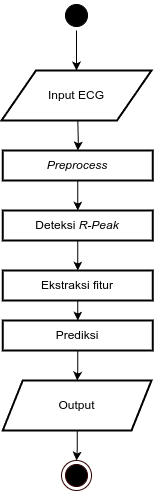
\includegraphics[width=.24\linewidth]{img/lstm-app flow.drawio.pdf}
	\caption{Diagram alir aplikasi inferensi}
	\label{fig:flowchart-inferensi}
\end{figure}

Gambar \ref{fig:flowchart-inferensi} menunjukkan alur kerja aplikasi inferensi yang dirancang.
% Setelah pengguna mengunggah data ECG, data tersebut akan melalui tahap \textit{preprocessing}, deteksi R-peak, ekstraksi fitur, prediksi, dan menghasilkan output hasil klasifikasi detak jantung.
Setelah pengguna mengunggah data ECG, aplikasi akan melakukan tahap \textit{preprocessing}, deteksi R-peak, ekstraksi fitur, klasifikasi, dan menghasilkan output hasil klasifikasi detak jantung.
Output tersebut akan ditampilkan pada antarmuka aplikasi inferensi yang dapat diakses oleh pengguna.
% Preprocessing dan deteksi R-peak penting dilakukan karena data rekaman ecg yang digunakan untuk inferensi belum terdapat anotasi pada titik R-peak.
Berbeda dengan tahap pelatihan, pada tahap inferensi, data ECG yang diunggah belum memiliki anotasi R-peak.
Oleh karena itu, perlu dilakukan tahap \textit{preprocessing} dan deteksi R-peak sebelum data dapat digunakan untuk klasifikasi detak jantung.

\begin{figure}[H]
	\centering
	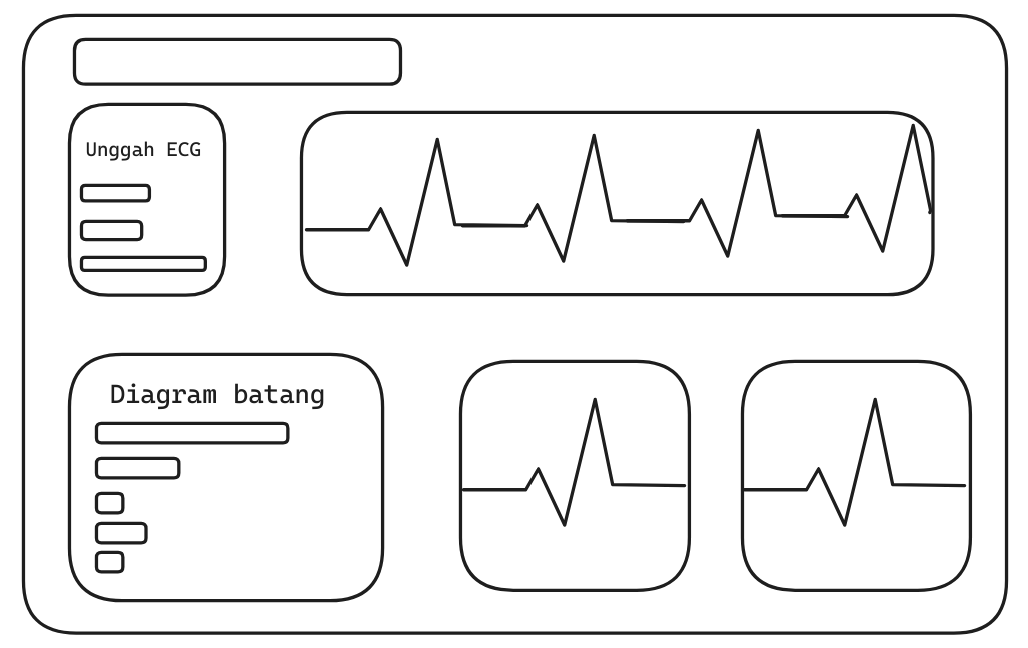
\includegraphics[width=.8\textwidth]{img/2024-06-24_12-19.png}
	\caption{Desain antarmuka aplikasi inferensi}
	\label{fig:lofi-inferensi}
\end{figure}

% --- perancangan antarmuka aplikasi
Gambar \ref{fig:lofi-inferensi} menunjukkan desain antarmuka aplikasi inferensi yang dirancang.
Antarmuka aplikasi terdiri dari dua bagian utama, yaitu bagian input dan bagian output.
Pada bagian input, pengguna dapat mengunggah data ECG yang akan digunakan untuk klasifikasi detak jantung.
Pengguna juga dapat memilih model yang akan digunakan untuk klasifikasi.
% Pada bagian output, dibagi menjadi tiga bagian, yaitu visualisasi data ECG, hasil klasifikasi berupa diagram batang, dan contoh sinyal ECG detak jantung pada setiap kelas.
Pada bagian output, terbagi menjadi tiga bagian.
Bagian pertama menampilkan visualisasi data ECG yang diunggah oleh pengguna.
Bagian kedua menampilkan hasil klasifikasi detak jantung dalam bentuk diagram batang.
Bagian terakhir menampilkan sampel sinyal ECG detak jantung pada setiap kelas yang telah diklasifikasikan oleh model.




